\documentclass[13pt]{extarticle}

\usepackage[utf8]{inputenc}
\usepackage[russian]{babel}

% page margin
\usepackage[top=0.5cm, bottom=0.5cm, left=1cm, right=1cm]{geometry}

% AMS packages
\usepackage{amsmath}
\usepackage{amssymb}
\usepackage{amsfonts}
\usepackage{amsthm}

\usepackage{float}
\usepackage{graphicx}
\usepackage{tabularx}
\usepackage[justification=centering]{caption}

\newcommand{\lb}{\left(}
\newcommand{\rb}{\right)}
\newcommand{\dprime}{{\prime\prime}}

\makeatletter
\setlength{\@fptop}{0pt}
\makeatother

\renewcommand{\arraystretch}{1.2}

\begin{document}

\title{Определение константы диссоциации азотной кислоты методом КР}
\date{}

\maketitle

\vspace*{-2cm}

\begin{figure}[!ht]
	\centering
	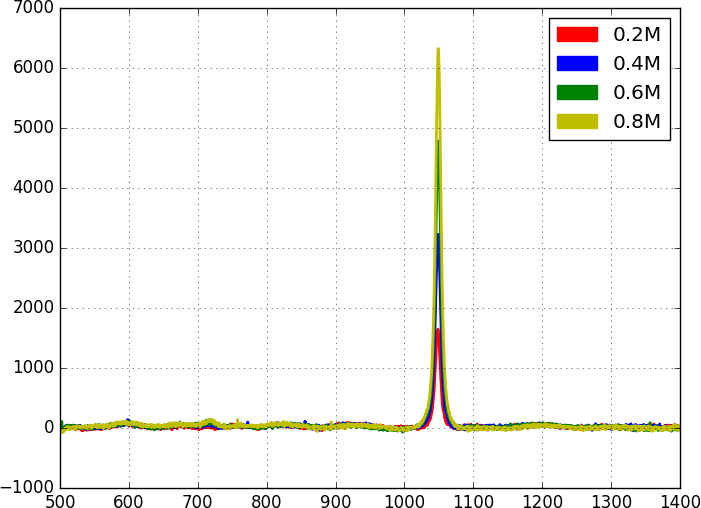
\includegraphics[scale=0.5]{../dilute.png}
	\caption{Спектры разбавленных растворов}
\end{figure}

\begin{figure}[!ht]
	\centering
	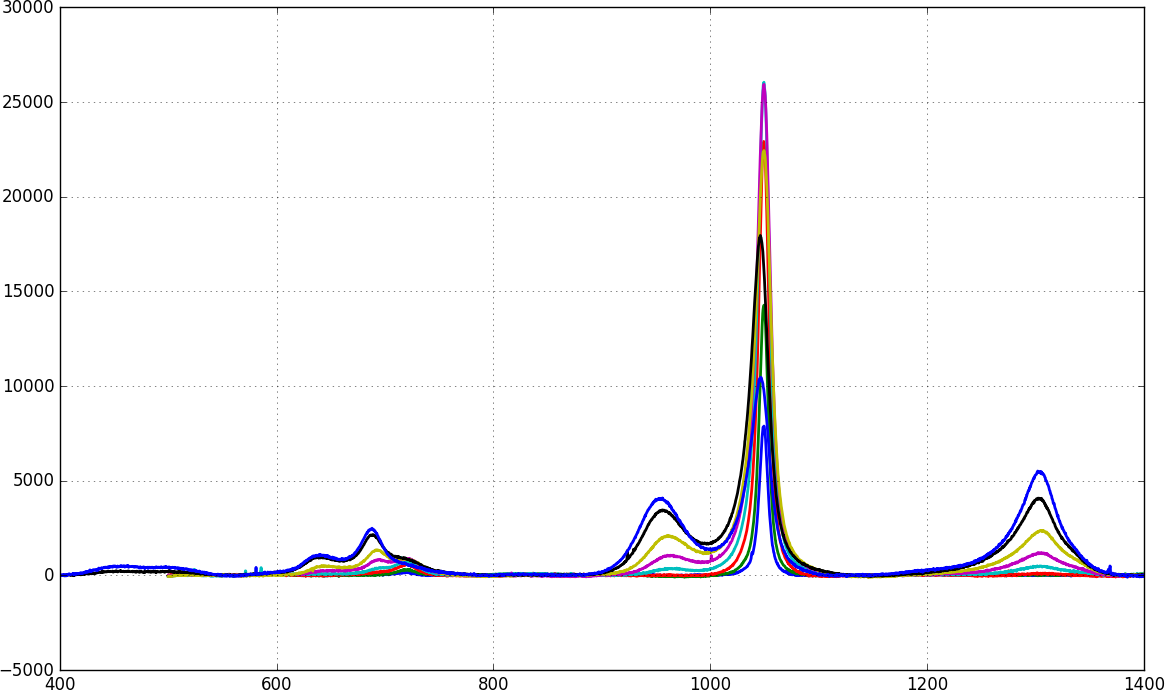
\includegraphics[scale=0.3]{../concentrated1.png}
	\hspace{0.5cm}
	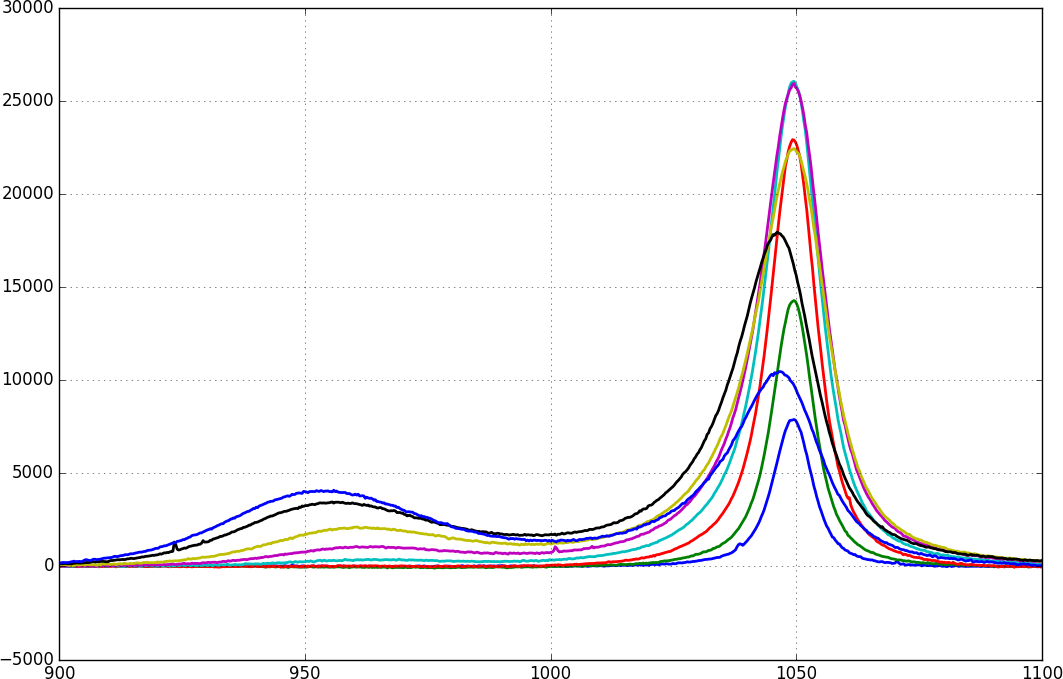
\includegraphics[scale=0.3]{../concentrated2.png}
	\caption{Спектры концентрированных растворов}
\end{figure}

\begin{figure}[!ht]
	\centering
	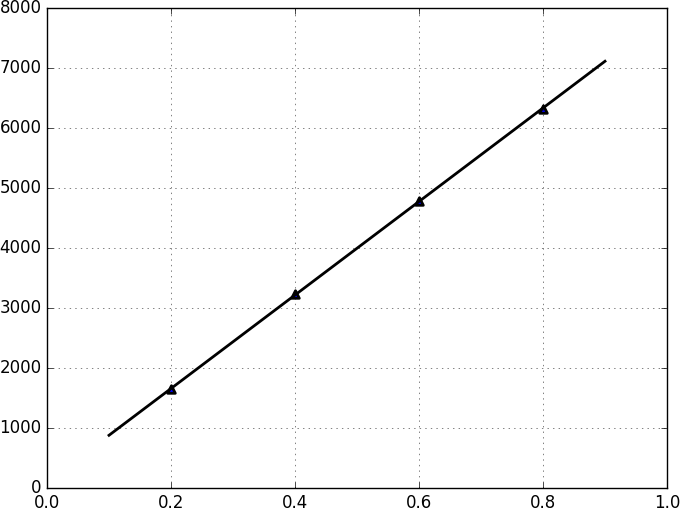
\includegraphics[scale=0.5]{../regr.png}
	\caption{Калибровочный график для определения нитрат-иона}
\end{figure}

\begin{gather}
	K_c = \frac{ [H^+][NO_3^-]}{[HNO_3]} = \frac{ [NO_3^-]^2 }{C(HNO_3) - [NO_3^-]} \notag
\end{gather}

\begin{figure}[!ht]
	\centering
	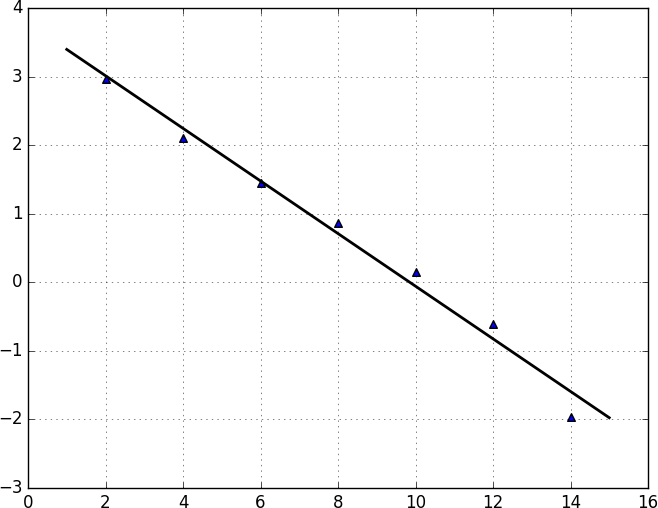
\includegraphics[scale=0.5]{../regr2.png}
	\caption{Зависимость $\ln K_c$ от $C(HNO_3)$}
\end{figure}

Экраполируя зависимость $K_c$ от $C(HNO_3)$ при $C(HNO_3) \rightarrow 0$, получаем термодинамическую константу диссоциации азотной кислоты:
\begin{gather}
	K_a = \lim_{C(HNO_3) \rightarrow 0} K_c = \exp ( b ) = 43.77 \notag
\end{gather} 


\end{document}